% This tallk should last between 10 and 15 minutes,
% and consist of 10 to 15 slides.
% I should cut back and forth between slides and actual pieces.
% I should leave  a little more than 5 minutes for questions.

\documentclass{beamer}

\mode<presentation>
{
  \usetheme{Warsaw}
  \definecolor{links}{HTML}{2A1B81}
  \hypersetup{colorlinks,linkcolor=,urlcolor=links}
  %\usetheme{Frankfurt}
  \usecolortheme{seagull}
  % or ...
  \setbeamercovered{transparent}
  % or whatever (possibly just delete it)
}

\usepackage[english]{babel}
\usepackage[utf8]{inputenc}
\usepackage{times}
\usepackage[T1]{fontenc}
\usepackage{fancyvrb}
\usepackage{listings}
\usepackage{graphicx}
\usepackage{attachfile}
\usepackage{ifthen}

\setbeamertemplate{caption}[numbered]
%\numberwithin{figure}{section}

\newboolean{localPieces} %Declaration, defaults to false
\setboolean{localPieces}{false} %Assignment

\title[cloud-5] % (optional, use only with long paper titles)
{cloud-5: \\\
A System for Composing and Publishing Cloud Music}

\author[Gogins] % (optional, use only with lots of authors)
{Michael Gogins \\ \url{http://michaelgogins.tumblr.com} }
% - Give the names in the same order as the appear in the paper.
% - Use the \inst{?} command only if the authors have different
%   affiliation.

\institute[Irreducible Productions] % (optional, but mostly needed)
{
  Irreducible Productions\\
  New York
}
% - Use the \inst command only if there are several affiliations.
% - Keep it simple, no one is interested in your street address.

\date[18 September 2024] % (optional, should be abbreviation of conference name)
{18 September 2024}
% - Either use conference name or its abbreviation.
% - Not really informative to the audience, more for people (including
%   yourself) who are reading the slides online

\subject{Computer Music}
\expandafter\def\expandafter\insertshorttitle\expandafter{%
    \insertshorttitle\hfill%
    \insertframenumber\,/\,\inserttotalframenumber}
% This is only inserted into the PDF information catalog. Can be left
% out. 
\begin{document}
\lstset{basicstyle=\ttfamily\tiny,commentstyle=\ttfamily\tiny,tabsize=2,breaklines,fontadjust=true,keepspaces=false,fancyvrb=true,showstringspaces=false,moredelim=[is][\textbf]{\\emph\{}{\}}}

\begin{frame}
  \titlepage
\end{frame}

\begin{frame}{Introduction}
\begin{itemize}
\item cloud-5 is a new system for composing, performing, and publishing computer music, using only Web standards.
\item In this talk, I focus on the \emph{motivations} for creating cloud-5.
\item Implementation details may be found in my \href{https://github.com/gogins/michael.gogins.studio/blob/master/music/ICSC-2024/cloud-5.pdf}{paper}, and in the \href{https://github.com/gogins/cloud-5}{cloud-5 GitHub repository}.
\item I show how cloud-5 accommodates composing, live performance, and online publishing in one environment. 
\end{itemize}
\end{frame}

 % \tableofcontents
  % You might wish to add the option [pausesections]

\section{Motivations}

\begin{frame}{Motivations}
\begin{itemize}
\item \emph{Primarily} I want to make the kind of music that I like to hear, but nobody else seems to be making, using algorithmic composition and synthesis.
\begin{itemize}
\item As I wander down this thorny path, I find myself wanting to perform some pieces live.
\item I also find myself wanting to make some pieces that play indefinitely, that are "always on."
\item And to generate visuals \emph{from} my pieces, or to transform visuals \emph{into} pieces.
\end{itemize}
\item \emph{Secondarily}, I need to drastically cut time spent maintaining software:
\begin{itemize}
\item By using Web standards to run identically on all platforms...
\item ...which simplifies my software infrastructure.
\item ...and simplifies online publication.
\end{itemize}
\end{itemize}
\end{frame}

\begin{frame}{Fundamental Dilemma}
\begin{itemize}
\item My \emph{tertiary} motivation is ongoing changes in how music is disseminated.
\begin{itemize}
\item If musicians use social media to publish music, it will be captured by social media (e.g.YouTube and SoundCloud) in order to gather personal data from them and their audience, to sell for targeted advertising.
\item This is annoying, and social media have cut mechanical royalties to practically nothing.
\item Social media also promote stylistic conformity and ghettoization.
\end{itemize}
\end{itemize}
\end{frame}

\begin{frame}{}
\begin{itemize}
\item Yet if musicians want to avoid capture by advertisers, difficulties arise:
\begin{itemize}
\item On some social media, musicians can avoid ads, but only by paying for subscriptions.
\item There are only a few social media that are free of both ads and subscriptions, but they are not popular.
\item Musicians can avoid social media altogether, but only by setting up their own Web sites.
\end{itemize}
\item Fortunately, setting up personal Web sites has gotten easier and cheaper over time.
\item And if musicians do create their own Web sites, that opens up wonderful new possibilities.
\end{itemize}
\end{frame}

\begin{frame}{Online Music}
\begin{itemize}
\item Music on a Web site doesn't need to be streamed from files -- \emph{it can be Web pages actually generating music in real time}.
\item Writing pieces as Web pages makes it possible to use all the resources of contemporary Web browsers.
\item Within its security sandbox, \href{https://html5test.co/}{a browser is basically an operating system plus a fast general-purpose programming language plus a game engine plus a high-resolution media player}.
\item Therefore, Web standards do not impose any particular limitation on audio quality, or other technical aspects (except for local file access), as compared with native applications.
\end{itemize}
\end{frame}

\begin{frame}{Cloud Music}
\begin{itemize}
\item I call music that is played by Web pages on the World Wide Web \emph{cloud music} because it exists only in the cloud, the omnipresent computing infrastructure of the World Wide Web.
\item I feel it is very important to grasp that cloud music is essentially \emph{a new medium for music} and as such,\emph{ it offers new possibilities of musical expression}.
\begin{itemize}
\item A piece can simply be an \href{http://localhost:8000/cloud5-example-score-generator.html}{algorithmically generated piece of fixed duration}, "tape music."
\item A piece can \href{http://localhost:8000/cloud_music_no_2.html}{generate visuals}.
\item \href{http://localhost:8000/cloud_music_no_1.html}{Visuals can generate music}.
\item A piece can \href{http://localhost:8000/cloud5-example-visual-music.html}{interact} with its listener.
\item Listeners can use a piece to \href{http://localhost:8000/cancycle.html}{create new pieces}.
\item \href{http://localhost:8000/cancycle.html}{A piece can play indefinitely (or not).}
\end{itemize}
\end{itemize}
\end{frame}

\begin{frame}{New possibilities}
\begin{itemize}
\item cloud-5 is certainly not the first system for publishing music as Web pages on the World Wide Web:
\begin{itemize}
\item \href{https://gibber.cc/playground/}{Gibber}, for live coding.
\item \href{https://strudel.cc/}{Strudel}, for live coding.
\item \href{https://ide.csound.com/}{Web-IDE}, for online Csound pieces.
\item ...and many others.
\end{itemize}
\item These systems support multiple users, and provide a playground for shared learning and experimentation.
\item By contrast, cloud-5 is designed to host \emph{permanent} pieces that use algorithmic composition and synthesis \emph{at a high level of power...}
\item\emph{ ...yet with low overhead for development and maintenance.}
\end{itemize}
\end{frame}

\section{Design}
\begin{frame}{Design}
\begin{itemize}
\item The cloud-5 system is a combination of:
\begin{itemize}
\item The sound processing language \href{https://csound.com/}{Csound}, compiled from C to WebAssembly.
\item The live coding system \href{https://strudel.cc}{Strudel}, written in JavaScript.
\item The algorithmic composition system \href{https://github.com/gogins/csound-ac/blob/master/README.md}{CsoundAC}, compiled from C++ to WebAssembly.
\item \href{https://www.shadertoy.com/}{GLSL shaders}.
\end{itemize}
\item Each component comes with its own JavaScript API, which cloud-5 encapsulates in custom HTML elements.
\item All libraries, assets, and all other pre-requisites are \emph{static resources} on the server filesystem.
\item There is no build system for pieces.

\end{itemize}
\end{frame}

\section{Composing}

\begin{frame}{Composing}
\begin{itemize}
\item A cloud-5 piece is a Web page written with a text editor.
\item A high-level menu system provides the shell for a piece; menu items show/hide overlays.
\item The composer writes code (JavaScript, Csound, Strudel, GLSL...) to fill out, connect, and control custom elements.
\item A naming convention makes it clear what composers need to add to the elements in order to make actual pieces.
\item The computer music \href{https://github.com/gogins/csound-ac/tree/master/vscode-playpen}{playpen} extension for Visual Studio Code enables editing any code in a piece, and immediately playing that revision from a local Web server.
\item The versionless nature of Web standards means pieces should remain playable into the indefinite future.
\end{itemize}
\end{frame}

\begin{frame}{Example}
\begin{figure}
\centering
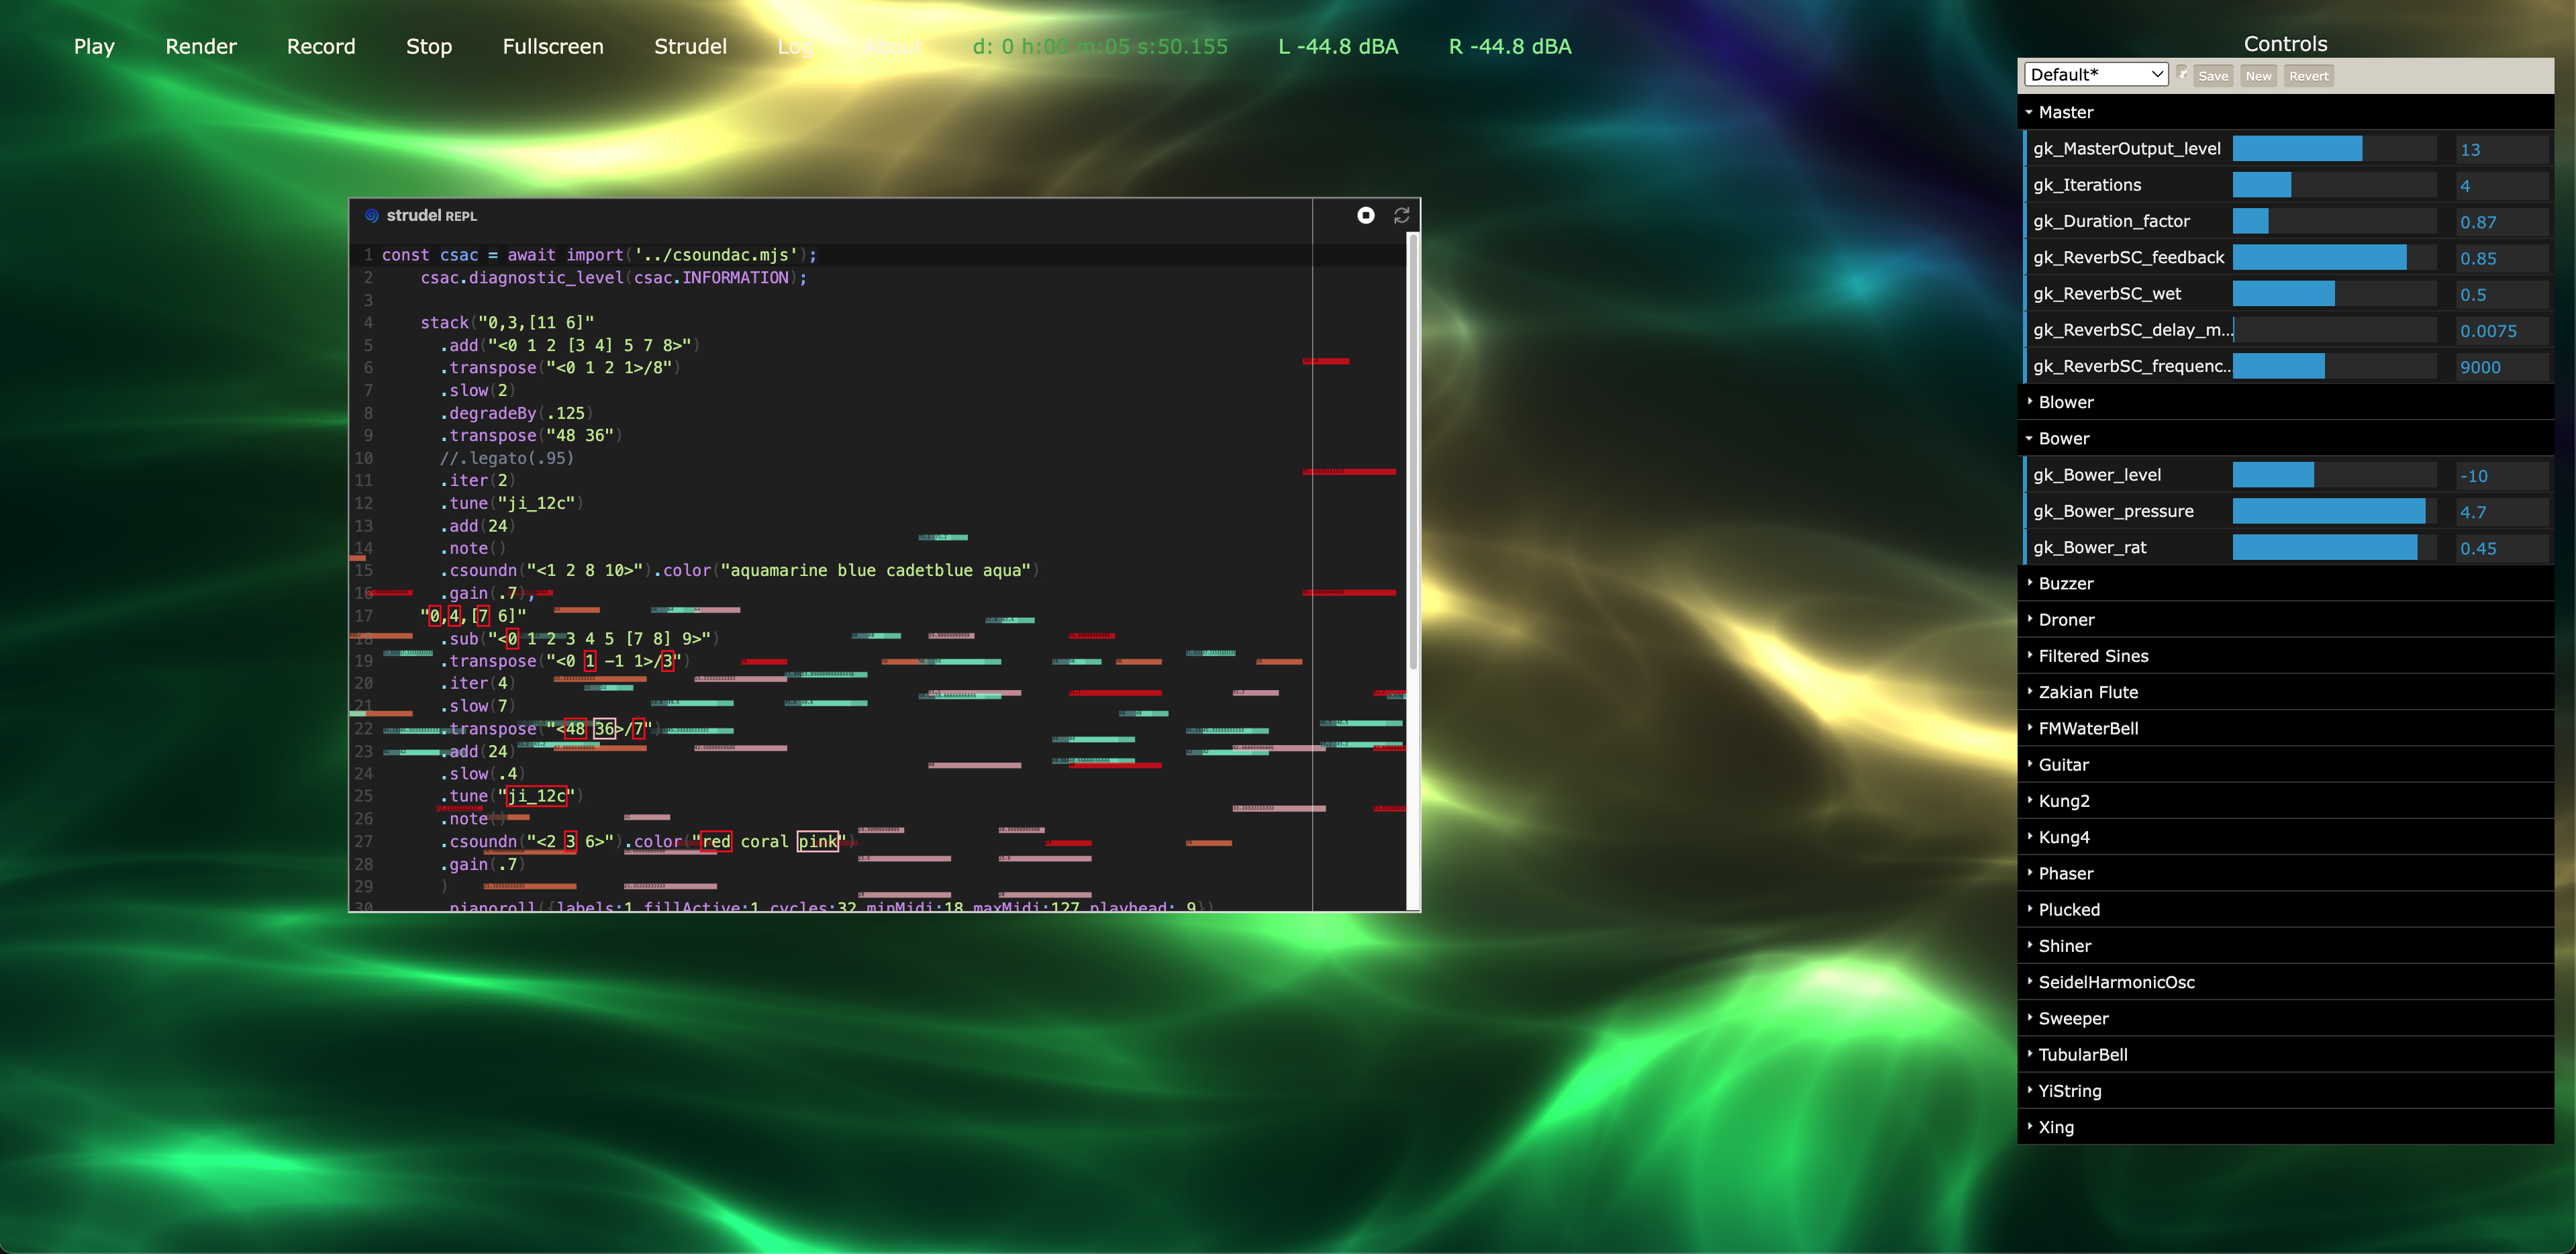
\includegraphics[width=0.90\linewidth]{cloud5}
\caption{cloud-5 Piece with Strudel and Audio Visualization}
\label{fig:cloud5}
\end{figure}
\end{frame}

\begin{frame}{}
\begin{figure}
\centering
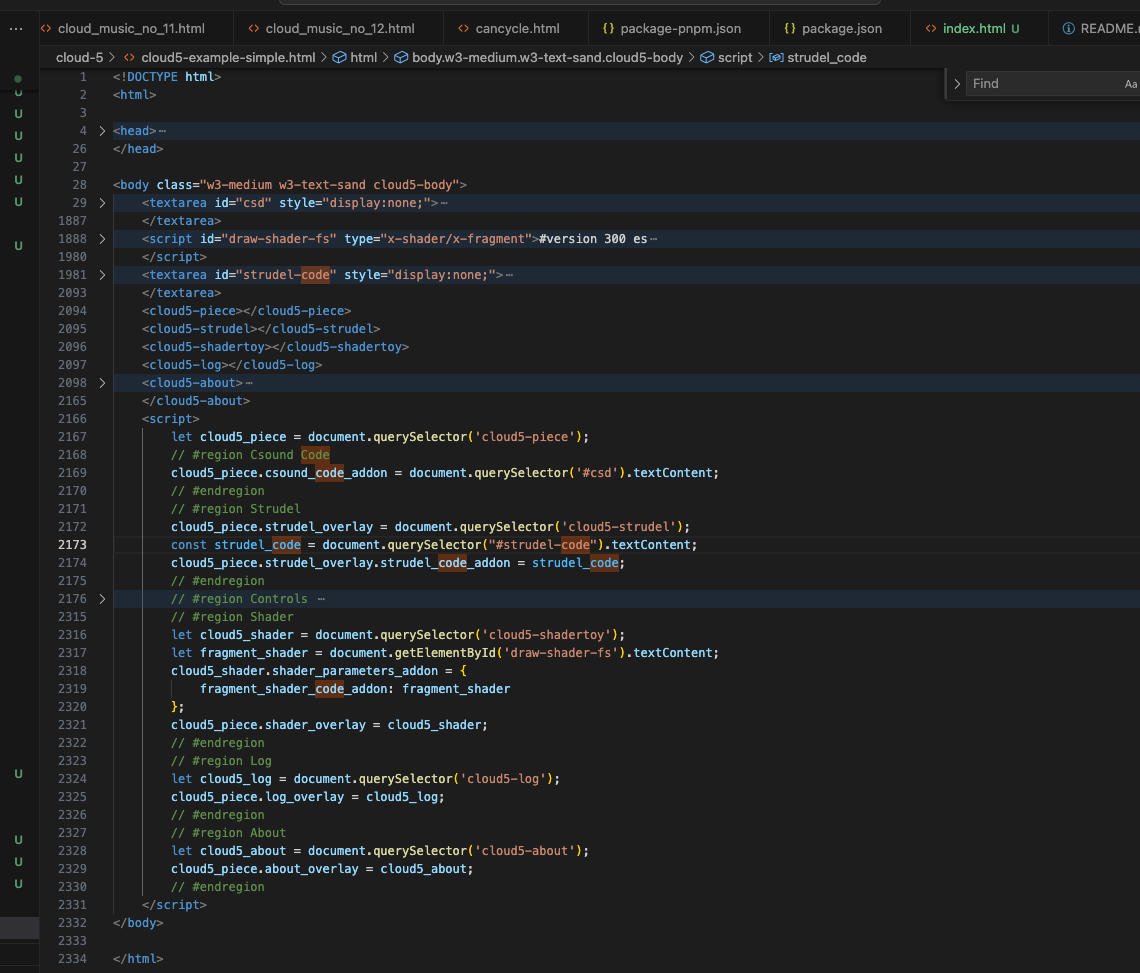
\includegraphics[height=0.85\textheight]{cloud5-code}
\caption{Outline of code}
\label{fig:cloud5-code}
\end{figure}
\end{frame}

\begin{frame}{Publishing}
\begin{itemize}
\item Copy the cloud-5 directory to any Web server. It contains all the libraries and assets that you need.
\item The cloud-5 directory can be the server's root directory, or it can be a subdirectory.
\item The Web server can be a local server for writing pieces or performing live pieces, or a server hosted on the Internet for publishing pieces online.
\item Musical compositions, of course, are simply Web pages in the cloud-5 directory.
\item Write the index page of your Web server to list and link to pieces to be published.
\item \href{https://gogins.github.io}{Period}.
\end{itemize}
\end{frame}

\end{document}


